
%
% ---- Chapter layout ----
%
% 1) Introduction - 
% 2) 
% ------------------------



\chapter{Biogenic Isoprene emissions in Australia} % Chapter title
\label{BioIsop}
  
%----------------------------------------------------------------------------------------
% Section 1 -- INTRO 
%----------------------------------------------------------------------------------------
\section{Introduction}  
\label{BioIsop:intro}  
  
  
  
  % isoprene and Australia
  Australian forests are strong emitters of both isoprene and monoterpenes.
  However emissions are poorly understood due to poor measurement coverage.
  The lack of measurements makes it difficult to estimate important subsequent processes such as ozone and secondary organic aerosol (SOA) formation.
  Isoprene has a large impact on the oxidative properties of the atmosphere, as it reacts quickly with the OH radical.
  One frequently used model of biogenic volatile organic compound (BVOC) emissions is MEGAN \parencite{Guenther2000} which estimates $\sim 1150$\tgpyr globally.
  The primary BVOC emission is isoprene, globally modelled at $\sim$465-500\tgcpyr \parencite{Guenther2006, Messina2016}. 
  The emission models used to derive these estimates are estimate fluxes from different plant species (phenotypes), which are seldom well understood within Australian forests.
  Isoprene emissions may be overestimated in Australia since they are based on measurements of taken from a few heavily emitting young eucalyptus trees which are not representative \parencite{Winters2009, FortemsCheiney2012,}.
  
  Satellite based emissions estimates allow us to improve the models without requiring other expensive measurements over the large data sparse continent of Australia.
  %%BVOC emissions are rising globally, and improving estimates for Australia is a priority since they affect such important processes in the atmosphere.
  \textcite{Kefauver2014} reviews remote sensing of BVOC emissions, examining the last 20 years of data and analysis of the satellite products.
  Their review reinforces the message that BVOCs affect the oxidative capacity of the atmosphere and are largely driven by and sensitive to vegetation.
  In the troposphere, BVOC emissions affect the hydroxyl radical (OH) cycling, ozone (O$_3$) and secondary organic aerosol (SOA) production, and methane longevity.
  The chemistry involved is complex and still suffers from relatively large uncertainties in both measurement and chemistry mechanisms.
  
  In this chapter the we use and describe a technique using satellite measurements of HCHO to estimate surface isoprene emissions.
  In-situ isoprene concentration measurements are costly and sparse within Australia, while satellite HCHO data are plentiful and freely available, making this technique very attractive.
  Such techniques have informed isoprene emission inventories in North America \parencite{Abbot2003,Palmer2003,Palmer2006,Millet2006,Millet2008}, South America \parencite{Barkley2013}, Europe \parencite{Dufour2009,Curci2010}, Africa \parencite{Marais2012}, Asia \parencite{Fu2007,Stavrakou2014}, India \parencite{Surl2018}, and even globally \parencite{Shim2005,FortemsCheiney2012,Bauwens2016}.
  HCHO is the dominant product of most BVOCs and is measured by remote sensing.
  HCHO products can be found in four satellite instruments: GOME on ERS-2, SCIAMACHY on ENVI-SAT, OMI on EOS AURA, and GOME2 on MetOp-A.
  These satellites have slightly different spectral and spatial resolutions, as well as using varied processes to estimate HCHO from detected radiances.
  This leads to different estimates between instruments as described in \textcite{Lorente2017}, and both validation and comparison become more important when using these remotely sensed data.
  In this thesis the OMHCHO dataset from the OMI instrument (see section \ref{Model:omhcho}) is used as the basis for HCHO amounts.
  
  
  \subsection{Aims}
    
    In a prior chapter (chapter \ref{Model}), the OMI HCHO total columns are recalculated using an updated estimate of HCHO profiles from GEOS-Chem v10.01 .
    These estimates are compared to available datasets of isoprene or HCHO (SPS1, SPS2, MUMBA, Wollongong FTIR). %, Daintree) 
    Sensitivity satellite AMF calculation is examined and quantified for some scenarios.
    In this chapter we outline why current isoprene emissions estimates are inadequate and how they can be improved.
    We discuss literature which shows how the estimates may be too high, and describe how emissions may be calculated using satellite datasets.
    Section \ref{BioIsop:method} lays out how new isoprene emissions are estimated, with results examined in Section \ref{BioIsop:results}. 
    In section \ref{BioIsop:conclusions} we examine how these changes in emissions would affect ozone concentrations in Australia, along with some other chemical processes.
    Uncertainties for each step along the way are quantified in section \ref{BioIsop:uncertainty}.
    
    %% AIMs paragraph
    Recent work suggests that modelled emissions may be overestimated in southeastern Australia, while emissions of monoterpenes (C$_{10}$H$_{16}$, two units of isoprene) appear to be underestimated \parencite{Emmerson2016}. 
    This could lead to the unique scenario of neither emission type dominating VOC chemistry over the forests.
    This work tries to improve the understanding of isoprene emissions over the whole of Australia, clarifying the spatial distribution of bias and how these biases impact modelled chemistry.
    We estimate isoprene emissions in Australia using top-down estimates based on OMI HCHO measurements and modelled isoprene to HCHO yields.
    This a posteriori top-down estimate is used to determine if model fit against sparse available ground-based measurements can be improved.
    GEOS-Chem model output is examined before and after updating isoprene emissions which are used as inputs.
    Wellness of fit between in-situ (at Wollongong) HCHO, satellite (OMI), and modelled (GEOS-Chem) HCHO is determined with and without updated emissions estimates.
    
  \subsection{Top-down isoprene emissions estimates}
    
    % Brief isoprene to hcho description
    In the remote troposphere HCHO production is dominated by methane oxidation, while in the continental boundary layer (CBL) production is largely due to non-methane VOCs (NMVOCs) \parencite{Abbot2003, Kefauver2014}.
    This leads to the technique of using a linear regression between enhanced HCHO and NMVOC emissions.
    In the CBL, HCHO enhancement is generally driven by short lived ($<1$~hr) precursors (most importantly isoprene).
    HCHO itself has a lifetime of a few hours \parencite{Kefauver2014}.
    Isoprene is emitted and enters the atmosphere in the gas phase, where it begins a complex series of reactions.
    Formaldehyde is produced with high yields in many of the isoprene reactions, which are discussed in more detail in Section \ref{LR:VOCs:IsopCascade}.
    HCHO measurements are often used as a check on how well isoprene reactions are simulated, as model output can then be compared against them \parencite{Marvin2017}.
    
    % First isoprene inversion work
    We broadly follow the method of \textcite{Palmer2001} to create an emissions estimate of isoprene over Australia.
    In their work isoprene emissions fluxes were derived using the Global Ozone Monitoring Experiment (GOME) satellite instrument, however here we use OMI (on board the AURA satellite) as it has better temporal coverage and increased pixel counts.
    Palmer's method improved biogenic isoprene emissions estimates (compared with in-situ measurements) over two available inventories: the U.S. EPA Biogenic Emissions Inventory System (BEIS2) and the Global Emissions Inventory Activity (GEIA).
    Here we try to improve MEGAN emissions estimates over Australia and analyse some of the technique sensitivities.
    
    Recently \textcite{Bauwens2016} estimated isoprene emissions with a top-down technique using the IMAGESv2 global CTM.
    They calculate emissions which create the closest match between model and satellite vertical columns, and compare these a posteriori data with their a priori (satellite data) and independent data sets.
    They examine global emissions seen by three models and a top-down inversion, showing a wide range of estimated values for Australia.
    In this thesis we prioritise the analysis of a top-down emissions estimate compared against MEGAN, along with flow on effect of changed emissions on modelled ozone levels.
    
    %    Top-down emission estimation is an in-depth process, and a couple of examples are provided here.
    %    \textcite{Marais2014} compare OMI based isoprene emission estimates against relaxed eddy accumulation measurements from African field campaigns in order to improve MEGAN emission factors in the region.
    %    \textcite{Dufour2009} use HCHO from SCIAMACHY, and examine Europe using CHIMERE as the chemical model, showing that satellite measurements can reduce source emission uncertainty by a factor of two, where emissions are relatively large.
    %    There are two main methods of estimating isoprene emissions using satellite measurements of child products, here I describe them and briefly compare the pros and cons of each.
    %    
    \subsubsection{Bayesian}
    
      % Top down emissions estimation methods:
      Bayesian inversion corrects biased biogenic isoprene emissions by optimising emission parameters in order to reduce the difference between observed HCHO and model output.
      In-depth inversions can account for effects from transport and allow source attribution \parencite{FortemsCheiney2012}.
      
      
      For example this method is used by \textcite{Shim2005} who optimise GEOS-Chem isoprene emissions in areas with high HCHO concentrations to improve comparison against GOME HCHO observations % They looking at areas with high signal to noise ratio (higher HCHO concentrations).
      They show that the original model underestimates isoprene emissions and HCHO concentrations by 14-46\%, with the corrected VOC emissions reducing model biases to 3-25\%.
      The Bayesian inversion is also used in \textcite{Curci2010}, where a regional CTM (CHIMERE) simulates HCHO, which is compared against OMI observed HCHO and shown to be regionally biased.
      %The CHIMERE model is used to derive yields of HCHO from the various local VOCs and these are then used in estimating local emissions.
      The model is run initially with emissions of BVOCs and reactive anthropogenic VOCs turned off in order to work out the background (b) values of these compounds.
      \textcite{Curci2010} uses CHIMERE as the forward model to determine the relationship between HCHO (y), isoprene and reactive anthropogenic VOCs (\textbf{x}), using 
      \begin{equation}
      y=\mathbf{K}x + b + \epsilon
      \end{equation}
      where $\epsilon$ are the (assumed) independent errors in measurements.
      K is the Jacobian matrix determined from CHIMERE representing the sensitivity of y to the state variable x.
      This K matrix is used in conjunction with error covariance in x to determine the Maximum A Posteriori solution to calculate the optimal estimate of x. % ($\hat{x}$).
      
      The Bayesian method is computationally expensive due to the requirement that model runs take place using many permutations of changed inputs.
      An advantage of the Bayesian method is that it can account for pyrogenic and anthropogenic emissions rather than filtering them out.
      Biases may still arise due to errors in modelled emission estimation \parencite{Curci2010}.
      In this work we do not use the Bayesian method due to the heavy computational costs involved.
      
        
    
    \subsubsection{Linear}
      \label{BioIsop:intro:top_down_linear}
      
      This technique is the simplest, and is performed in this thesis.
      Using vertical columns of biogenic HCHO one can infer the local (grid space) isoprene emissions using effective molar formaldehyde yield (In other continents around 2-3, or 1 in low NO$_X$ conditions) \parencite{Palmer2003,Marais2012,Bauwens2016}.
      If one assumes fast HCHO yield, so that the effect of chemical transport is minimal, and that HCHO and isoprene are at steady states, then one may calculate local yield from a CTM.
      %This yield is derived from both HCHO and isoprene, such as was used by \textcite{Millet2006} who produced a molar HCHO yield of 2.3 in north eastern USA.
      
      In this work yield is calculated from the modelled slope between isoprene emissions and HCHO tropospheric columns within each gridbox over Australia, as performed in \textcite{Palmer2003}, using modelled values between 1300-1400 LT which is around the overpass time of the OMI.
      This modelled yield is then used in conjunction with the recalculated OMI measurements in order to estimate isoprene emissions.
      To calculate this yield we use a reduced major axis (RMA) regression between modelled average values of the total columns and isoprene emission rates, an example is shown in figure \ref{BioIsop:intro:top_down_linear:fig_RMA_example} shows the modelled regression between emissions and tropospheric columns for January, 2005. Also shown is the time series for these two quantities averaged over Australia, and the squared correlation coefficient along with a sample from four gridsquares.
      The top down estimation process in this thesis is further explained in section \ref{BioIsop:method}.
      
      %Plot from GC_tests.py -> Examine_Model_Slope()
      \mypic{/Figures/OMI_link/GC/E_isop_vs_hcho_200501.png}{%
        Top left: RMA slope between modelled tropospheric column HCHO ($\Omega_{GC}$) and isoprene emissions ($E_{GC}$) using midday (13:00-14:00~LT) values over for January 2005, per gridsquare at 2x2.5\degr horizontal resolution.
        Top right: Australia-wide average of midday emissions and tropospheric columns.
        Bottom left: Squared RMA correlation coefficient for regression in top left. Coloured dots correspond to colour of regressions shown in bottom right panel.
        Bottom right: Sample of correlations from four gridsquares.}
      {\label{BioIsop:intro:top_down_linear:fig_RMA_example}}
      
      % Pros and cons:
      This technique suffers from the assumptions of fast HCHO yield and no transport, which requires filtering areas with low NO$_X$, high winds, or low emissions.
      Since we use an estimate of the yield from biogenic isoprene to HCHO, we must also filter out areas where HCHO may be coming from anthropogenic or pyrogenic sources.
      On the plus side, the simple nature of the inversion requires very little computational power after acquiring satellite and model datasets, even over large amounts of gridded data.
      Both the linear and Bayesian techniques assume that modelled chemistry is accurate and only try to correct precursor emissions, which may be a problem if the chemistry is uncertain.
      
      In high NO$_x$ environments where HCHO has a lifetime on the order of 30 minutes, it can be used to map isoprene emissions with spatial resolution from 10-100~kms.
      Horizontal transport \textit{smears} the HCHO signal so that source location would need to be calculated using wind speeds and loss rates \parencite{Palmer2001,Palmer2003}.
      Smearing requires analysis and filtering due to the importance of transport and NO$_X$ on forming robust and accurate estimates.
      Over Australia NO$_X$ levels are generally not high enough to ensure quick HCHO formation and we must take care to account for resultant smearing.
      Details on smearing analysis and filtering are in Section \ref{BioIsop:method:Smearing}.
    
      
  \subsection{MEGAN emission model}
    % Megan estimates BVOCs - uncertain
    The Model of Emissions of Gases and Aerosols from Nature (MEGAN) is one of the most popular emissions inventories for biogenic isoprene.
    Global atmospheric studies often use MEGAN along with a chemical transport model (CTM) to examine transport, emission, deposition, and other chemical processes in the atmosphere.
    Emissions of Biogenic Volatile Organic Compounds (BVOCs) including isoprene are often the subject of studies as they are still relatively uncertain, as well as being drivers for important oxidation and pollution events.
    In this work MEGAN is run as a module within GEOS-Chem, a global CTM which uses emissions inventories and meteorological data to simulate atmospheric gas concentrations and transport.
    
    MEGAN is poorly calibrated for Australian conditions.
    Emissions of isoprene (C$_5$H$_8$) may be overestimated in some regions within Australia.
    \textcite{Sindelarova2014} showed how the isoprene emissions could be as much as halved by accounting for lower soil moisture.
    \textcite{Stavrakou2015} saw isoprene emissions overestimated by a factor of 2-3 in January.
    \textcite{Emmerson2016} discuss the suitability of MEGAN's isoprene and monoterpene emission factors over southeast Australia, and suggest isoprene emissions are estimated 2-6 times too high.
    They also show that no blanket increase or decrease in emission factors is appropriate for the entire southeast of Australia.
    Additionally, emissions of monoterpenes (C$_{10}$H$_{16}$, two units of isoprene) appear to be underestimated \parencite{Emmerson2016}.
    This could lead to the unique scenario of neither emission type dominating VOC chemistry over the forests.
  
  
  \subsection{satellite measurements}
    \label{BioIsop:intro:satellite_inversion}
    % Lead in to satellite inversion
    Top-down estimates look at how much of a chemical is in the atmosphere and try to work out how much of its major precursors were emitted.
    This generally takes advantage of longer lived products which may reach a measurable equilibrium in the atmosphere.
    For isoprene this is done by looking at atmospheric HCHO enhancement, which can be largely attributed to isoprene emissions once transport and other factors are accounted for.
    %Even anthropogenic HCHO source estimates, which are accurate at the global scale, can be improved using satellite data to improve regional estimates by up to 25-40\% \parencite{Stavrakou2015}. 
    %Their study used the RETRO 2000 database for anthropogenic emission a prioris except for Asia in 2008 where REASv2 was used. 
    Since 1997, when GOME measurements were first used to measure HCHO over Asia \parencite{Thomas1998}, satellites have been used to provided a total column measurement of HCHO, allowing isoprene emissions estimates by proxy \parencite{Palmer2001,Bauwens2016}.
    Using satellite information to improve biogenic emissions is pinpointed as a valuable use of satellite derived datasets \parencite{Streets2013}.
    In this work we use NASA's OMHCHO product, using measurements from OMI on board the AURA satellite (see section \ref{Model:omhcho}).
    
    
    Satellites recording reflected solar spectra use DOAS to measure various trace gases in the atmosphere, including formaldehyde. 
    While satellite measurements can only be used during daytime hours, HCHO lifetimes are sufficiently short that any night-time chemistry will not affect midday observations \parencite{Wolfe2016}.
    %Satellites can be used to measure the seasonal and inter annual variability of HCHO over the globe.
    Satellite records are often compared with modelled estimates of HCHO and also used as a proxy to estimate isoprene emissions.
    Total HCHO is measured by satellite over the entire world.
    The technique used to determine precursor emissions suffers from uncertainties, not the least of which are the uncertainties in the satellite measurements themselves.
    \textcite{Zhu2016} use SEAC$^4$RS aircraft HCHO measurements over the southeastern US as model validation. 
    They show that a bias in the assumed OMI shape factor leads to a bias between satellite and SEAC$^4$RS measurements.
    Satellite based chemical concentrations often require both remote and in-situ measurements combined with modelled data for validation \parencite{Marais2014}.
    There is less information available from satellite measurements at higher latitudes due to increased error in measurements over the more slanted column paths \parencite{DeSmedt2015}.
    Validation is important due to the various uncertainties in the satellite remote sensing process, with a priori assumptions having the greatest effect on structural uncertainty between measurements techniques \textcite{Lorente2017}.
    
    
    
\section{Methods}
  \label{BioIsop:method}
  
  \subsection{Outline}
    % Method Briefly outlined here
    This sectin provides an overview of the steps involved in creating a top-down emissions estimate. %, from reading satellite data and model output to the creation of isoprene emissions estimates.
    This process is summarised in figure \ref{BioIsop:method:fig_Flow_Making_Isop}.
    \begin{enumerate}
      \item 
        Corrected vertical columns ($\Omega$; saved in OMHCHORP dataset) are calculated using level two OMI HCHO satellite data (see section \ref{Model:omhcho}), along with GEOS-Chem model runs (see section \ref{Model:GC:simulations}) at 0.25\degr by 0.3125\degr horizontal resolution (see section \ref{Model:omiRecalc}).
      \item 
        Level three satellite data are used to make anthropogenic, fire, and smoke influence masks (see section \ref{Model:Filter}).
        These are applied to remove $\Omega$ which may be influenced by non biogenic sources. 
      \begin{enumerate}
        \item 
          The fire mask is created daily from non-zero (MODIS) fire counts over the prior 2 days which occur in local or adjacent grid squares at 0.25\degr latitude by 0.3125\degr longitude
        \item 
          Influence from transported smoke plumes is removed by filtering OMI aerosol absorption optical depth (AAOD, from OMAERUVd) greater than 0.03
        \item 
          A filter for anthropogenic influence is created daily using OMNO2d NO$_2$ tropospheric column amounts; masking any grid squares with greater than $2\times 10 ^{15}$\moleccm2 on any particular day, along with grid squares where the yearly average is above $1.5 \times 10^{15}$\moleccm
      \end{enumerate}
      \item 
        GEOS-Chem modelled biogenic emissions of isoprene ($E_{GC}$) along with total biogenic columns of HCHO ($\Omega_{GC}$), both averaged over 2x2.5\degr horizontally  and 1300-1400~LT temporally, are used to calculate a linear regression slope ($\Omega_{GC}=S E_{GC} + \Omega_{GC;0}$)
        \begin{enumerate}
          \item 
            Hourly gridded model output $E_{GC}$~atoms C cm$^{-2}$ s$^{-1}$ is read, and 13:00~LT daily values are extracted.
          \item
            Daily 13:00-14:00~LT $\Omega_{GC}$\moleccm output is read.
          \item 
            A reduced major axis regression slope is determined between $\Omega_{GC}$ and E$_{GC}$ using a month of modelled output (one value per day) for each gridsquare (eg. see figure \ref{BioIsop:method:slope:fig_regressions})
        \end{enumerate}
      %\item For each of the corrected vertical columns (VCC$_{OMI}$, VCC$_{GC}$, and VCC$_{PP}$; see section \ref{Model:omiRecalc}), a top down estimate of biogenic isoprene emissions (E$_{new}$; atoms C cm$^{-2}$ s$^{-1}$) is calculated
      \item 
        $\Omega$ are used to create a top-down estimate of biogenic isoprene emissions ($E_{OMI}$~atoms C cm$^{-2}$ s$^{-1}$)
      \begin{enumerate}
        \item 
          Background total columns ($\Omega_{0}$) are calculated by averaging longitudinally the $\Omega$ between 180 and 120\degr W
        \item
          Emissions are calculated using 
          \begin{equation} \label{BioIsop:method:eqn_Enew}
            E_{OMI} = \frac{\Omega - \Omega{0}}{S}
          \end{equation}
      \end{enumerate}
      \item
        Modelled slope (S) calculations depend on several assumptions which are not always valid.
        A mask is created for where the HCHO production is not dominated by local isoprene emissions. 
        This is determined by calculating smearing over Australia using two model runs with differing isoprene emissions.
        This smearing value is determined as $\hat{S}=\Delta \Omega_{GC}/ \Delta E_{GC}$: the ratio of the differences between model runs of HCHO columns and isoprene emissions.
        The acceptable range for $\hat{S}$ over Australia is determined as 800 - 4600~s.
        A full description of the creation of this smearing filter is given in section \ref{BioIsop:method:Smearing}
      \item 
        Top-down emissions $E_{OMI}$ are compared against MEGAN estimated emissions, as well as analysed in conjunction with concentration measurement campaigns (MUMBA, SPS, and one set of airplane measurements (HIPPO)).
        TODO: do these things
      \begin{enumerate}
        \item 
          Top-down isoprene emissions are calculated for the time window 1300-1400~LT, matching the peak of the diurnal cycle
        \item 
          A monthly scaling factor ($\alpha$) for isoprene emissions is created based on the difference between peak MEGAN emissions and our top-down estimates
        \item GEOS-Chem is run using the a posteriori emissions, and HCHO, O$_3$, isoprene, and NO$_X$ outputs are compared to campaign measurements
      \end{enumerate}
    \end{enumerate}
    
    \mypic{Figures/Flow_Making_Isop.png}{Creation of isoprene emissions dataset using OMHCHORP and biogenic GEOS-Chem outputs.}{\label{BioIsop:method:fig_Flow_Making_Isop}}
  
  \subsection{Masks and reprocessed satellite HCHO}
    
    Satellite data pixels are read from the OMHCHO level 2 satellite dataset, AMFs are recalculated, and then pixels are gridded daily into 0.25x0.3125\degr horizontal bins. 
    This forms the intermediate product OMHCHORP, which is fully described in section \ref{Model:omiRecalc:outline}.
    %In total a month of these data are read in at a time %(to allow parallelism and reduce RAM usage)
    %and then used in subsequent steps to calculate the isoprene emissions.
    This dataset includes gridded satellite HCHO columns ($\Omega$), along with pixel counts (how many satellite datapoints were used for each gridbox) to allow averaging and resolution changes.
    
    In order to determine biogenic HCHO enhancements from $\Omega$, we require filters for non-biogenic sources.
    Anthropogenic, fire, and smoke influence masks are created from three satellite products: NO2 from OMNO2d, fire counts from MOD14A1, and AAOD from OMAERUVd respectively (see section \ref{Model:Filter}).
    These masks are binned using daily averaged or summed values within our 0.25x0.3125\degr horizontal resolution.
    The recalculated corrected vertical columns are saved to OMHCHORP dataset both before and after applying the filters, to allow filter analysis.
    While one primary source of HCHO production is methane oxidation, the linear regression used to estimate isoprene emissions effectively ignores this source as part of the background, which means a methane filter is not required.
    
    
  \subsection{Calculating modelled slope}
    \label{BioIsop:method:slope}
    
    % determination of HCHO = S E_isop + HCHO_BG
    By assuming a simple linear steady-state relationship between HCHO and its precursors \parencite{Palmer2003, Palmer2006, Millet2006}, one may calculate isoprene emissions using measured HCHO.
    The calculation requires reaction rates and yields from isoprene to HCHO, which can be determined most readily using chemical modelling.
    The methodology for calculating isoprene emissions from HCHO is laid out in \textcite{Palmer2003}, and takes into account the expected lifetime and reaction rates of the precursor VOCs and HCHO.
    Assuming HCHO is produced quickly from short-lived intermediates:
    \begin{eqnarray*}
      VOC_i \overset{k_i}{\rightarrow} Y_i HCHO
    \end{eqnarray*}
    Where $i$ indexes a chemical species, $Y_i$ is HCHO yield per C atom, and $k_i$ is the reaction rate.
    Then assuming a steady state of atmospheric HCHO ($\Omega$) in \moleccm produced by oxidation of VOCs (VOC$_i$) and no horizontal transport:
    \begin{eqnarray*}
      \Omega = \frac{1}{k_{HCHO}} \sum_{i} Y_i E_i
    \end{eqnarray*}
    Where $k_{HCHO}$ is the HCHO loss rate due to OH and photolysis, Y$_i$ is the molar HCHO yield from oxidation (of $i$), and $E_i$ is emission fluxes (C atoms $cm^{-2} s^{-1}$).
    We assume isoprene is the most important precursor and lump other terms into the background $\Omega_0$ so that our equation becomes 
    \begin{eqnarray} 
    \label{BioIsop:method:slope:eqn_isop_to_hcho}
    \begin{split}
      \Omega_{HCHO} 
      &= \frac{Y_{isop}}{k_{HCHO}} \times E_{isop} + \Omega_0 \\
      & = S \times E_{isop} + \Omega_0
    \end{split} \end{eqnarray}
    
    The equations above come from several assumptions that are important to understand.
    The first assumption is that HCHO %and isoprene ($I$)?
    is at steady state, which implies productions and losses are equivalent.
    Then we assume that loss is only due to photolysis and oxidation (first order, $k_{HCHO} = 1/\tau_{HCHO}$).
    Production of HCHO above a background is due to the sum of the precursor emissions ($E_i$) multiplied by their yields to HCHO ($Y_i$).
    \begin{eqnarray*}
      \frac{d [ HCHO ] }{dt} & = 0 = Prod(HCHO) - Loss(HCHO) \\
      Loss(HCHO)  & = k_{HCHO} [ HCHO ] \\
      Prod(HCHO)  & = \Sigma_i Y_i E_i  \\
    \end{eqnarray*}
    Now instead of concentrations we use total column amounts for HCHO, with emissions being in units of molecules cm$^{-2}$ s$^{-1}$.
    And then lumping together non-isoprene precursors, and assuming that enhancements above the background are only due to isoprene emissions we have: 
    \begin{eqnarray*}
    k_{HCHO} \Omega_{HCHO} & = Y_{isop} E_{OMI} + \Sigma_{i \ne isop} Y_{i} VOC_{i} \\
    \Omega_{HCHO} & = S E_{OMI} + \Omega_{0}
    \end{eqnarray*}
    
    
    Estimates of $Y_{isop}$ or $S$ can be attained through modelling \parencite[e.g.][]{Millet2006}.
    We look at each $2\times2.5$~\degr grid box from daily GEOS-Chem (biogenic only) output of $\Omega_{HCHO} \equiv \Ogc$ and $E_{OMI} \equiv E_{GC}$ within Australia, and calculate the (RMA) correlation for each month.
    Modelled background concentrations can be ignored here as they do not affect slope calculation.
    This effectively gives us monthly gridded isoprene to HCHO slope ($S$) in units of molecules HCHO $/$ atom C $\times$ seconds (seconds).
    Figure \ref{BioIsop:method:slope:fig_regressions} (top left) shows the RMA regression slope between modelled HCHO columns and isoprene emissions calculated within each grid square over January 2005, averaged between 1300-1400~LT each day.
    Also shown are the regression coefficients (bottom left), Australia averaged $E_{GC}$ and $\Ogc$ time series (top right), and a sample of the regressions (bottom right).
    Each regression is for a single grid box, over the course of one month, and is coloured by location (matching dots shown in the bottom left panel).
    The slopes shown in the bottom right panel can range widely due to differences in emission and yield parameters, which plays a role in the smearing filters applied in section \ref{BioIsop:method:Smearing}.
    Due to the low horizontal resolution of GEOS-Chem (2 by 2.5\degr, latitude by longitude), calculations from grid boxes on the coast which are largely oceanic need to be discarded as the change in HCHO is not dominated by emissions of isoprene, as is assumed for equation \ref{BioIsop:method:slope:eqn_isop_to_hcho}.
    
    
    \mypic{Figures/OMI_link/GC/E_isop_vs_hcho_200501.png}
    { % Caption
      Top left: the RMA regression slope between modelled HCHO columns and isoprene emissions calculated within each grid box over January 2005.
      Bottom left: the square of the regression coefficients.
      Top right: Australia averaged time series 
      Bottom right: a sample of the regressions coloured by latitude and longitude pairs, matching dots in the bottom left panel.
    }
    {\label{BioIsop:method:slope:fig_regressions}}
    
    
    %%A nested version of GEOS-Chem would allow better analysis of coastal regions, at 0.25 by 0.3125$^{\circ}$ resolution, however this may require more explicit handling of smearing.
    %\begin{figure}
    %  % Figure from GC_tests.py -> isop_hcho_RMA
    %  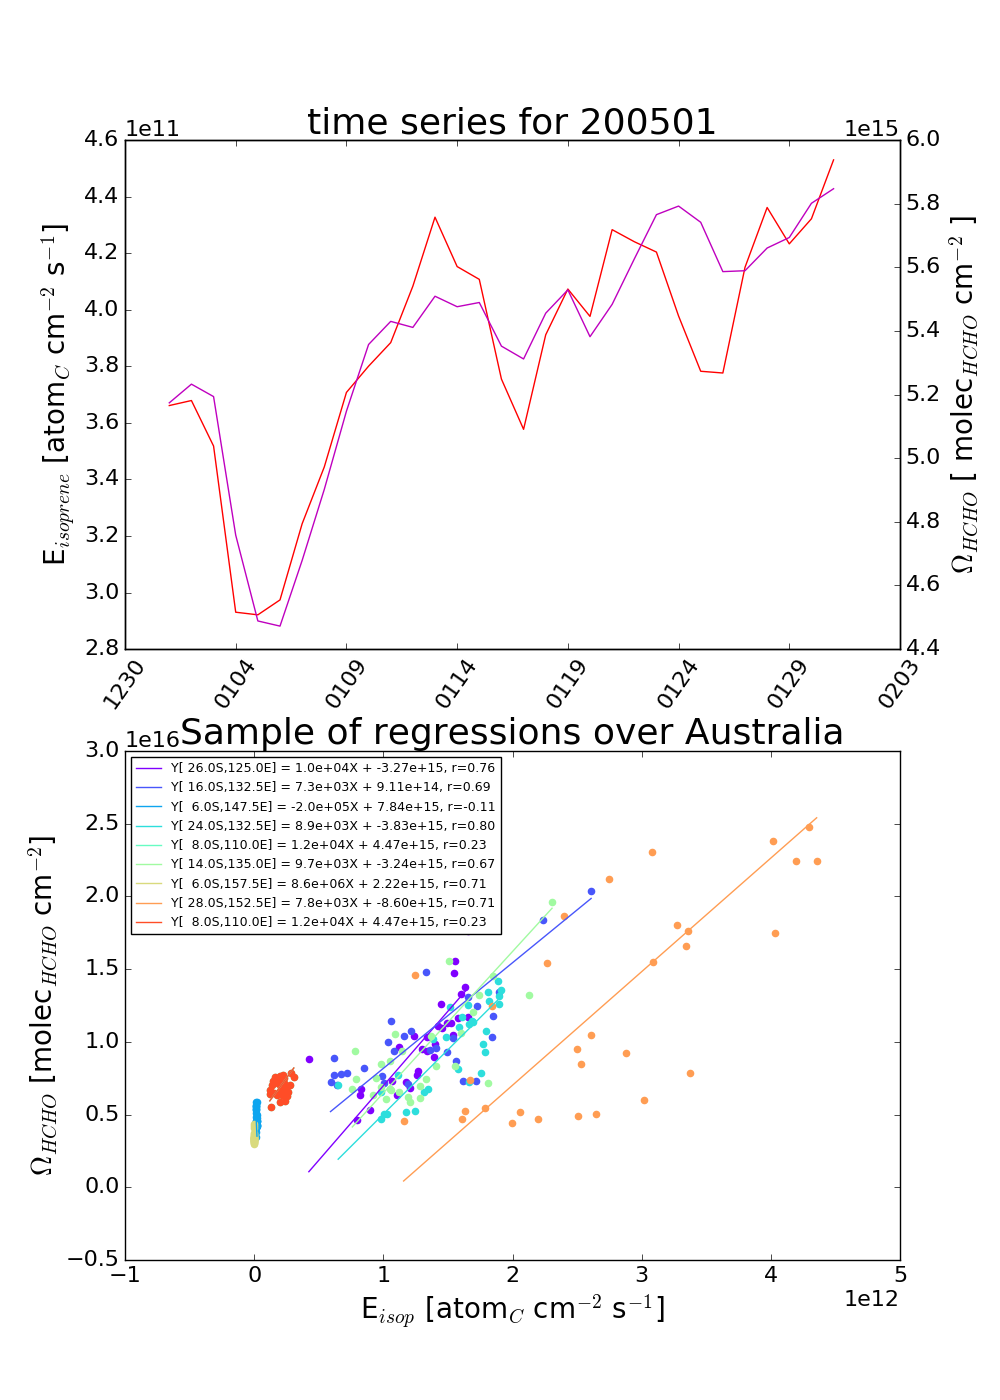
\includegraphics[width=\textwidth]{Figures/Isoprene/E_isop_vs_hcho_series_200501.png}
    %  \caption{%
    %    Top panel: isoprene emissions for January, 2005, shown in red, co-plotted with tropospheric hcho columns, shown in magenta.
    %    Both series are daily averages over Australia.
    %    Bottom panel: (RMA) linear regressions from between emissions of isoprene and tropospheric hcho columns, sampled randomly from the 2$^{\circ}$ by 2.5$^{\circ}$ latitude longitude gridboxes over Australia for the month of January (2005).
    %  }
    %  \label{BioIsop:method:calculation:fig_E_isop_vs_hcho_model_sample}
    %\end{figure}
    
    %% BACKGROUND calculation(s)
    There are a couple of ways to determine the modelled background HCHO concentration, one of which involves running the model with isoprene emissions turned off, which allows us to see exactly how much the modelled isoprene emissions alter each vertical column of HCHO.
    This is effective since we have assumed variation in HCHO columns only depends on isoprene emissions, so our background term is theoretically identical to the emission free simulated HCHO.
    The other way involves looking at HCHO over the remote pacific at matching latitudes and times, which emulates how the background is determined for the satellite measured HCHO.
    Figure \ref{BioIsop:method:fig_background_hcho} shows GEOS-Chem total column HCHO with and without isoprene emissions along with amounts over the remote pacific at the same latitudes.
    Background HCHO for any latitude in this thesis are calculated by averaging longitudinally (140\degr W to 160\degr W) the matching latitudes over the remote pacific.
    %These backgrounds are used when creating the reference sector corrections for satellite measurements (in section \ref{Model:omiRecalc:RSC}).
    %The background columns are longitudinally averaged from 140\degr W to 160\degr W.
    
    
    \mypic{Figures/OMI_link/GC/GC_background_hcho_200501.png}{Total column HCHO over Australia (left) and the remote pacific region (right) using GEOS-Chem with (top) and without (bottom) isoprene emissions. }{\label{BioIsop:method:fig_background_hcho}}
    
    
  \subsection{Calculation of Emissions}
    \label{BioIsop:method:calculation}
   
    % First: outline of what we do
    As is done in \textcite{Palmer2003, Millet2006, Bauwens2016}, we assume that HCHO and isoprene columns are in a steady state, with no horizontal transport.
    We also assume that isoprene is the only compound enhancing the HCHO levels, which requires that we filter out influence from fires, smoke, and anthropogenic emissions.
    Emissions of precursors are easy to calculate using the slope $S$ calculated in the prior section from modelled HCHO and isoprene columns:
    \begin{equation*}
    \Omega = S \times E_{OMI} + \Omega_0
    \end{equation*}
    This is the same equation \ref{BioIsop:method:slope:eqn_isop_to_hcho}, except now we use the modelled slope along with satellite HCHO ($\Omega$, and $\Omega_0$).
    The background HCHO is calculated using measurements in the remote pacific at the same time and latitude as $\Omega$.
    This leaves $E_{OMI}$ as the only unknown once the satellite measurements are processed to match the temporal and horizontal resolution of $S$.
    Figure \ref{BioIsop:method:calculation:fig_E_isop_200501} shows the emissions calculated this way along with the modelled emissions output by GEOS-Chem $E_{GC}$ averaged over January, 2005.
    \begin{figure}
      % Figure from Analyse_E_new.MEGAN_vs_E_new()
      \includegraphics[width=\textwidth]{Figures/OMI_link/Emiss/MEGAN_vs_E_VCC_PP_lr_20050101-20051231.png}
      \caption{%
        Top row is isoprene emissions for the month of January, in 2005, from GEOS-Chem and estimated from OMI respectively.
        Bottom row shows the absolute and relative differences between the two.
      }
      \label{BioIsop:method:calculation:fig_E_isop_200501}
    \end{figure}
    
    %% How we use the background..
    The Background ($\Omega_0$) from OMI is determined using the mean column HCHO measured over the remote pacific ocean.
    For this term we use remote ocean measurements averaged monthly and longitudinally.
    This is gives us a background which is appropriate for any latitude.
    Figure TODO: figure with background region highlighted and a time series of background values.
    One potential issue is the low number of valid measurements at high latitudes (especially during winter).
    When calculating the $E_{OMI}$ from our modelled slope, negative emissions result when using OMI measured columns are lower than the background amounts (as $E_{OMI} = \frac{\Omega - \Omega_0}{S}$).
    These are set to zero, which increases the average by TODO: $\sim$X~\%.
    
    Top-down emission rates calculated in this work are in units of molecules cm$^{-2}$ s$^{-1}$.
    In order to calculate the emissions in kg, each gridsquare is multiplied by the area, and then daily emissions are assumed to follow a sine wave peaking at the estimated rate.
    Figure \ref{BioIsop:method:calculation:fig_daily_emissions_kg} shows how the daily approximation of total emitted isoprene per grid square is calculated. 
    Daytime hours are estimated per month, from 14~hrs (Jan) to 10~hrs(Jul).
    
    
    \mypicw{0.5\textwidth}{Figures/Emissions_per_day.png}{%
      How daily isoprene emissions (in kg) are calculated.
    }{\label{BioIsop:method:calculation:fig_daily_emissions_kg}}
  
  \subsection{Accounting for smearing}
    \label{BioIsop:method:Smearing}
    
    Accounting for transport of the precursors is important, especially in low NO$_X$ conditions in which isoprene has a longer lifetime (hours-days).
    When estimating emissions of isoprene using one of its products, it is often assumed that isoprene has a short lifetime.
    This is a problem in Australia where low NO$_X$ environments abound, as detected formaldehyde may not be directly above its emission source (as assumed in this top-down estimation technique).
    An analysis of spatial smearing (smearing from here forwards) can be used to mitigate potential emissions estimation biases by filtering out affected gridsquares.
    Smearing in this case is a measure of how much formaldehyde is created from isoprene emissions in non-local grid boxes.
    Smearing has been estimated in various works \parencite[eg.][]{Martin2003, Palmer2003, Millet2006, Stavrakou2009, Marais2012, Barkley2013, Zhu2014, Wolfe2016, Surl2018}, often implementing the method designed in \textcite{Palmer2003}.
    This method involves calculating smearing using two almost identical model runs, one of which has isoprene emissions scaled globally by a factor (generally from 0.5 to 2).
    Another method \parencite[eg.][]{Stavrakou2009} involves the analysis of an adjoint CTM, however this is computationally expensive.
    
    In this work a run of GEOS-Chem using globally halved isoprene emissions (with no other changes) is performed to create a smearing filter.
    Consider halving the isoprene emitted globally and rerunning the model, one would expect HCHO enhancement (above background levels) to be halved in isoprene emitting gridboxes if no transport has occurred.
    This idea is behind the method of testing the correlation between HCHO enhancement and isoprene emissions.
    By assuming no transport and negligible yield and lifetime changes between model runs, an equation can be derived and tested, finding where the assumptions lead to unlikely yields.
    
    
    In order to filter potential smearing, a daily modelled value for $\hat{S} \approx Y_{isop}/k_{HCHO}$ is determined.
    By assuming midday HCHO lifetime typically falls within 1.5 to 4~hrs (as seen in the USA), and isoprene to HCHO yield (HCHO per isoprene carbon emitted) lies within the range 0.2 to 0.4 (scenarios estimated in \textcite{Palmer2003}): one can set a simple bound on $\hat{S}$ of $[0.2 \times 1.5, 0.4 \times 4]$~hrs or 1080 to 5760 seconds.
    As NO$_X$ levels across Australia are relatively low, the yield is likely lower than seen in \textcite{Palmer2003}: and here we reduce the bounds by 20\% and round to the nearest hundred to get a bounding range of 800 to 5200 for $\hat{S}$. 
    This range strikes a balance between unlikely modelled yields and how much data is lost to filtering.
    A better approximation of lifetimes for HCHO is required to properly account for seasonality and regional NO$_X$ concentrations.
    TODO: Figure todo shows $\hat{S}$ over Australia for one year, along with where and when the filter has most impact.
    %Todo?: Show yield and lifetimes from caaba/mecca if possible
    Table \ref{BioIsop:method:Smearing:tab_smearing_ranges} shows the smearing filters or typical slopes seen in other works.
    
    \begin{table}\begin{threeparttable}
      \caption{Smearing filters or slopes ($S$) seen in literature.}
      \begin{tabular}{ l | c  c  >{\centering\arraybackslash}p{5cm} } 
        \toprule
        Publication & min. (s) & max. (s) & Notes \\
        \midrule
        \textcite{Palmer2003}      & 1270 & 2090 & Slope ranges seen in North America Summer \\
        \textcite{Marais2012}      &      & 4000 & Smearing limits for Africa \\
        \textcite{Barkley2013}$^a$ & 1300 & 1800 & Smearing limits for South America \\
        \textcite{Surl2018}        & 2200 & 4900 & Slope ranges seen in India \\
        
        \bottomrule
      \end{tabular}
      \begin{tablenotes} 
        \item a: Assumed HCHO lifetime of 2.5 hours implies yields from 0.14 to 0.2 per C, consistent with box modelling.
        %\item b: In this work the slopes are shown 
      \end{tablenotes}
      \label{BioIsop:method:Smearing:tab_smearing_ranges}
    \end{threeparttable}\end{table}
    
    
    %\textcite{Marais2012} additionally use airborn isoprene, MVK $+$ MACR (isoprene oxidation products), and HCHO measurements to check smearing in Africa where there is a sharp gradient of isoprene emitting vegetation from north to south.
    
    \subsubsection{Calculation of smearing}
      \label{BioIsop:method:Smearing:calculation}
      
      % slope and yields
      In order to understand the smearing calculation the underlying equations and assumptions must first be understood.
      From section \ref{BioIsop:method:slope}, equation \ref{BioIsop:method:slope:eqn_isop_to_hcho} we have the formulation of a modelled slope (S) being the yield of HCHO per C of emitted isoprene divided by HCHO loss rate per second ($S = \frac{Y_{isop}}{k_{HCHO}}$).
      % smearing defined from two runs of geos chem
      Using two runs of GEOS-Chem with isoprene emissions being the only difference we have:
      \begin{eqnarray}
        \label{BioIsop:method:Smearing:calculation:eqn_runs}
        \begin{split}
        Run_1 :&  \Omega_{HCHO} = S E_{isop} + \Omega_0 \\
        Run_2 :&  \Omega_{HCHO}' = S' E_{isop}' + \Omega_0' 
        \end{split}
      \end{eqnarray}
      There are several assumptions which need to be understood, as these are what is tested by the smearing calculation.
      The initial assumption is that the system is in a steady state, with no transport of isoprene affecting HCHO columns, this is the basis for equations \ref{BioIsop:method:Smearing:calculation:eqn_runs}.
      It is assumed that background values ($\Omega_0$) are from oxidation of methane and other long lived VOCs, so that $\Omega_0 = \Omega_0'$.
      Between these two runs we are only changing the $E$ term, we do not change any chemistry and so we can expect that the yield and loss rate is not changing between the two runs $S = S' = \frac{Y_{isop}}{k_{HCHO}}$
      %    \begin{eqnarray*}
      %      S = S' & = \frac{Y_{isop}}{k_{HCHO}} \\
      %      \Omega_0 & = \Omega_0'
      %    \end{eqnarray*}
      which leads to us being able to combine the runs in equation \ref{BioIsop:method:Smearing:calculation:eqn_runs} as follows:
      \begin{eqnarray}
        \label{BioIsop:method:Smearing:calculation:eqn_hats}
        Run_1-Run_2 :& \Omega_{HCHO} - \Omega_{HCHO}' = S E_{isop} - S' E_{isop}' +\Omega_0 - \Omega_0' \\
        & \Delta \Omega_{HCHO} = S \Delta E_{isop} \\
        & \hat{S} \equiv \frac{\Delta{\Omega_{HCHO}}}{\Delta E_{isop}} \approx \frac{Y_{isop}}{k_{HCHO}}
      \end{eqnarray}
      And using the output from our two runs we can see if the calculated $\hat{S}$ is wildly different from expected values for S.
      %The modelled slope multiplied by the column HCHO loss rate ($k_{HCHO} = 1/\tau$) should approximate the HCHO yield from isoprene \parencite{Palmer2003, Barkley2013}.
      
      
      Similarly to smearing sensitivity calculations in \textcite{Marais2012}, we run GEOS-Chem with isoprene emissions halved, then calculate $\hat{S} = \frac{\Delta \Omega_{HCHO}}{\Delta E_{isop}} $.
      Here $\Delta$ represents the departure (daily over 1300-1400~LT) from default run values.
      If $\hat{S}$ is large, then you can infer sensitivity to non-local isoprene emissions.
      A relatively large change in $\Omega_{HCHO}$ compared to local emissions suggests that HCHO is being formed from non-local isoprene emissions.
      Alternatively a relatively low value of $\hat{S}$ infers that emissions from a particular grid square are being exported before they form HCHO, which also informs us that local HCHO levels are not due to local emissions.
      
      Smearing is sensitive to how E$_{isop}$ is determined, figure \ref{BioIsop:method:Smearing:fig_smearing_def_2005} shows smearing over two seasons defining E$_{isop}$ as the daily averaged (left column) and midday (1300-1400~LT) isoprene emissions (right column). 
      Essentially the midday isoprene emissions are at the peak of their daily cycle (shown later in figure \ref{BioIsop:method:scaled:megan_diurnal}) which means the effect of smearing is relatively smaller during these hours.
      Figure TODO: shows averaged isoprene emissions with added markers showing when the threshold of 800-5200 affects at least one day within the season (cyan or pink diamonds) and where it removes all data for that gridbox (blue or red x).
      
      
      \mypic{/Figures/OMI_link/Filters/smearing_definitions_2005.png}{Smearing ($\hat{S}$, see text) in summer (DJF, top row) and winter (JJA, bottom row) using averaged isoprene emissions daily (left column) and 1300-1400~LT (right column). The scale changes between left and right columns.}{\label{BioIsop:method:Smearing:fig_smearing_def_2005}}
      
      
      % Marais 2012 also look at average windspeed and best hcho-isop corelation when hcho is shifted by 0.5 degrees, don't think I can do that with 2.5 degree resolution
      % Marais compare smearing with model estimated yield "

    \subsubsection{Sensitivity to smearing}
    
      Smearing can be dependent on local or regional weather patterns, as greater wind speeds will reduce the time any emitted compound stays within the local grid box.
      As such smearing sensitivity is both spatially and temporally diverse.
      Figure TODO: is a picture of the smearing sensitivity over Australia in Summer and Winter, along with where the smearing threshold is exceeded (for one or all days).
      Large smearing values can be seen near many coastlines as only a fraction of the grid squares actually emit isoprene, which makes transported isoprene relatively more important in these gridboxes.
      Once the smearing sensitive grid squares are filtered out, application of equation \ref{BioIsop:method:slope:eqn_isop_to_hcho} is used to estimate isoprene emissions across the nation.
      
      %TODO: Plots of S hat showing worst smearing affected areas per season.
      
      
      % TODO: figure out this paragraphs numbers, make plot
      When limiting smearing ($\hat{S}$) to within 800-4600~s, GEOS-Chem correlation between isoprene emissions and HCHO columns should improve (TODO analysis). 
      A problem arises due to the loss of datapoints used to create monthly gridsquare regressions, and a secondary filter is applied where the confidence interval of the slope exceeds 200\%.
      Figure TODO shows GEOS-Chem midday HCHO columns compared against GEOS-Chem emissions of isoprene, over land squares with (red) and without (grey) filtering for smearing.
      This smearing range captures isoprene to HCHO yields of around 0.16 to 0.32 C per C if HCHO lifetime is assumed to lie within 1.5 to 4 hours.
    
    \subsubsection{Smearing length scale}
    
      The expected horizontal transport (prior to reaction) of a precursor can be calculated using the smearing length \parencite{Palmer2003}.
      The distance travelled (L) downwind (d) by a precursor (i) before becoming HCHO can be estimated through:
      \begin{equation*}
        L_{d,i} = \frac{U}{k_i - k_{HCHO}} \ln{ \left( \frac{k_i}{k_{HCHO}} \right) }
      \end{equation*}
      where U is wind-speed.
      \textcite{Palmer2003} further define a smearing length scale: L$_{s,i}$ as the distance downwind where a fraction (1 - $1/e$) of the precursor is completely transformed into HCHO.
      This equation uses the initial VOC column concentration ($[VOC]_0$) at the point of emission and mass balance equations as follows:
      \begin{equation}
      \frac{1}{k_{HCHO}-k_i} \left( k_{HCHO} \exp{ \left[ \frac{-k_i L_{s,i}}{U} \right]} -k_i \exp{ \left[ \frac{-k_{HCHO} L_{s,i}}{U} \right]} \right) = \frac{1}{e} 
      \end{equation}
      with limiting values L$_{s,i} \rightarrow U/k_i$ for $k_i << k_{HCHO}$, and L$_{s,i} \rightarrow U/k_{HCHO}$ for $k_{HCHO} << k_i$.
      Figure TODO: shows a rough estimate of isoprene smearing length(L$_{isop}$) in Australia using wind speeds from TODO:, and reaction rates k$_{isop}$, k$_{HCHO}$ from GEOS-Chem.
      %TODO make this plot!
      
      GEOS-Chem daily averaged HCHO lifetime ($\tau$) is shown for 2005 in figure \ref{BioIsop:method:Smearing:fig_tau_GC_2005}.
      This lifetime is calculated using daily averaged surface loss rates and concentrations of HCHO:
      \begin{equation*}
      \tau = \frac{[HCHO]}{Loss}
      \end{equation*}
      The expected lifetime of HCHO is determined by assuming loss is linear (first order) and dividing grid box daily averaged concentrations of GEOS-Chem HCHO ($[HCHO]$ in molecules cm$^{-3}$) by their modelled losses ($Loss$ in molecules cm$^{-3}$ s${-1}$).
      For each grid square over Australia this daily averaged surface lifetime in summer (Jan., Feb.) and winter (JJA) is shown in figure \ref{BioIsop:method:Smearing:fig_tau_GC_2005}.
      Additionally lifetimes coloured by land grid squares (dots in top right panel) are shown over time in the bottom panel.
      The problem with this approximation is that we are not interested in daily averaged lifetime, but the midday (13:00-14:00~LT) lifetime.
      This figure highlights the seasonal nature of HCHO loss rates, although midday numbers are expected to have less seasonality.
      Another highlighted issue is the potential latitudinal dependence of HCHO lifetimes, since there is less total insolation leading to lower HCHO loss rates at higher latitudes.
      
      
      \mypic{/Figures/OMI_link/Filters/tau_2005.png}{%
        Top left, right: Summer (Jan., Feb.) and winter (JJA) averaged daily surface HCHO lifetime ($\tau$). Bottom panel: $\tau$ over the year, coloured by grid square (see dots in top right panel).
      }{\label{BioIsop:method:Smearing:fig_tau_GC_2005}}
      
    
    \subsubsection{NOx dependence}
      
      Isoprene production of HCHO depends on several factors, importantly NO$_X$ levels directly affect the fate of VOCs in the atmosphere.
      Isoprene first reacts with the hydroxy radical, producing an organic peroxy radical (RO$_2$).
      At higher NO mixing ratios (at least a few hundred pptv), RO$_2$ react mostly with NO. 
      At low NO (less than 50~pptv), RO$_2$ is more likely to either isomerise, or react with HO$_2$, or another RO$_2$.
      In low NO$_X$ environments, reported HCHO yields from isoprene are around 0.2 - 0.3 C per C, while in high NO$_X$ environments this value becomes two to three times higher \parencite{Palmer2003, Wolfe2016}.
      %\textcite{Wolfe2016} also see background HCHO doubling in high NO$_X$ regions.
      %\textcite{Wolfe2016} determine that going from NO$_X = 0.1$ to $2.0$ ppbv triples the prompt yield of HCHO, from 0.3 to 0.9 ppbv ppbv$^{-1}$ due to isoprene, while the background HCHO doubles.

      
      NO$_2$ measured by OMNO2d gives us a daily mid-day measurement which we can compare to output from GEOS-Chem to determine how well the model does at simulating NO$_2$ (see section \ref{Model:GC:NOx}).
      %\textcite{Travis2016} show how NO$_X$ can be used to examine model bias in ozone (potentially due to NO$_2$ bias) over the USA.
      The affect of NO$_2$ on smearing can be seen in figure \ref{BiogIsop:Method:smearing:fig_smearing_vs_nox}.
      This plot shows how smearing over Australia compares to satellite NO$_2$ levels, with smearing distributions binned by NO$_2$ both with and without applying a filter for smearing.
      One feature of the figure is that at lower NO$_2$ levels the smearing is often 2-4 orders of magnitude above the upper threshold. 
      This abruptly decreases at around $5 \times 10^{14} $~molec cm$^{-2}$ NO$_2$.
      There is also a higher number of data points below the lower threshold before that same NO$_2$ level, suggesting that transport is a bigger issue at NO$_2 < 5 \times 10^{14} $~molec cm$^{-2}$. 
      
      %% FIGURE SHOWS SMEARING BINNED BY NOX
      % Figure made in test_filters.smearing_nox() 
      \mypic{Figures/OMI_link/Filters/smearing_nox_200501.png}{%
        Top left: OMNO2d tropospheric NO$_2$ columns (NO$_2$: molec cm$^{-2}$) averaged into 2x2.5\degr horizontal bins for over Jan, 2005.
        Right: Scatter plot of NO$_2$ against smearing calculations from GEOS-Chem ($\hat{S}$), with points above and below the smearing threshold range of 900-5200~s coloured red and blue respectively. Points are binned by NO$_2$ with and without having the smearing filter applied (orange and magenta respectively). Overplotted is the mean and standard deviation (error bars) within each bin. Due to the logarithmic Y scale we only show the positive direction of standard deviations for unfiltered data.
        Bottom left: Daily NO$_2$ scattered against smearing with (magenta) and without (orange) applying the smearing filter. This plot is a zoomed out version of the right panel.
      }{\label{BiogIsop:Method:smearing:fig_smearing_vs_nox}}
      
      The half-life of HCHO to photo-oxidation with hydroxyl radicals is around 1~hr depending on environmental conditions \parencite{WHO_hcho_guidelines_2010}.
      This would make the expected lifetime ($\tau = \text{half-life}/\ln{2}$) around 1.4 hours.
      Over the majority of Australia conditions are relatively clean (low NO$_X$ levels) which extends the expected lifetime.
      The estimated loss rate of HCHO in GEOS-Chem %approximately ranges from 1e6 to 3e6 mol cm$^{-3}$ s${-1}$, 
      is up to three times higher in summer and along the north and eastern regions associated with denser forest regions, when compared against other regions.
      This is largely due to loss rates being proportional to concentrations.
      %Isoprene yields from various sources are shown in table \ref{BioIsop:method:tab_VOCAusYields}.
      %\textcite{Wolfe2016} determine that going from NO$_X = 0.1$ to $2.0$ ppbv triples the prompt yield of HCHO, from 0.3 to 0.9 ppbv ppbv$^{-1}$ due to isoprene, while the background HCHO doubles.
      
      Conversions between HCHO per unit C yield and molar \% yield from species X are given by the equation $ Y_{molar \%} = 100 \times C_X \times Y_{HCHO \,C^{-1}}$, where $C_X$ is how many carbon are within species X (5 for isoprene).
      For instance a 200\% molar yield of HCHO from isoprene implies 1 mole of C$_5$H$_8$ becomes 2 mole HCHO which is a 0.4 HCHO per unit C yield.
      
      %    TODO: Fill out this table
      %    \begin{table} \begin{threeparttable}
      %        \caption{HCHO yields from various species averaged over Australia during Summer.}
      %        \begin{tabular}{ | c  c  c  c  c | }
      %          \toprule
      %          \textbf{Species}   & \textbf{Emissions$^a$}& \textbf{Lifetime$^b$}& \textbf{HCHO Yield$^c$} & \textbf{HCHO production$^d$\%}
      %          \\                 & (Tg C per month)      &                      & (per C reacted)         &         \\
      %          \midrule
      %          Isoprene           & Y                     & n minutes            & 0.x                     & 10       \\
      %          $\alpha$-Pinene    & Y                     & n minutes            & 0.x                     & 10       \\
      %          $\beta$-Pinene     & Y                     & n minutes            & 0.x                     & 10       \\
      %          HCHO               & Y                     & n minutes            & 1.0                     & 10       \\
      %          \bottomrule
      %        \end{tabular}
      %        \begin{tablenotes} 
      %          \item a: Calculated using GEOS-Chem emissions over Australia in January 2005.
      %          \item b:  
      %          \item c: 
      %          \item d: Production determined by dividing emission*yield by the sum of all VOC emissions*yields. 
      %        \end{tablenotes}
      %        \label{BioIsop:method:tab_VOCAusYields}
      %      \end{threeparttable} \end{table}
      %      
      % yields from Atkinsen2003
      %isoprene
      %0.63 0.10 Tuazon and Atkinson (1990a)
      %0.57 0.06 Miyoshi et al. (1994)
      % a-pinene
      %0.23 0.09 Noziere et al. (1999a)
      %0.19 0.05 Orlando et al. (2000)
      % b-pinene
      %0.54 0.05 Hatakeyama et al. (1991)
      %0.45 0.08 Orlando et al. (2000)
      
      % molar HCHO yield per unit carbon equal to HCHO molar percent yield(per carbon)? or some conversion?
      \begin{table} \begin{threeparttable}
          \caption{ HCHO yields from isoprene, and lifetime against oxidation by OH. }
          \begin{tabular}{  l  l  l  l  }
            \toprule
             HCHO Yield    & Life vs OH   & NO$_X$ background & Source   \\
            (molar \% )   &              &                   &          \\
            \midrule 
             315$\pm$50      &            & High          & a        \\ 
             285$\pm$30      &            & High          & a        \\ 
             225             & 35 min     & High          & b        \\ % Done
             150             &            & Low           & b        \\ % Done
             150             &            & Low           & d        \\
             450             &            & High          & d        \\
             235             &            & 1~ppbv        & e        \\
             150             &            & 0.1~ppbv      & e        \\
            %          $\alpha$-Pinene & 28$\pm$3        &        & Low                & c        \\ 
            %          & X$\pm$3         &        & X                  & d        \\ 
            %          & 230$\pm$90      &        & High        & a        \\ 
            %          & 190$\pm$50      &        & High        & a        \\ 
            %          & 19              & 1 hour &              & b        \\ % Done
            %          & 210             &        & 1~ppbv        & e        \\
            %          & 70              &        & 0.1~ppbv      & e        \\
            %          $\beta$-Pinene  & 65$\pm$6        &        & Low           & c      \\ 
            %          & X$\pm$3         &        & X             & d      \\ 
            %          & 540$\pm$50      &        & High          & a     \\ 
            %          & 450$\pm$80      &        & High          & a      \\ 
            %          & 45              & 40 min &              & b      \\ % Done
            %          Methane 	      & 100             & 1 year  &             & b     \\ 
            %          Ethane          & 180             & 10 days &             & b     \\ 
            %          Propane         & 60              & 2 days  &             & b     \\ 
            %          Methylbutanol   & .13(per C)    & 1 hour  &             & b     \\ 
            %          HCHO            & 100             & 2 hour  &             & b     \\ 
            %          Acetone         & .67(per C)      & 10 days &             & b     \\ 
            %          Methanol        & 100             & 2 days  &             & b     \\ %Done
            \bottomrule
          \end{tabular}
          \begin{tablenotes} % \item makes new lines
            \item a \textcite{AtkinsonArey2003}: Table 2, Yield from Isoprene reaction with OH, two values are from two referenced papers therein.
            \item b \textcite{Palmer2003}: lifetimes assume [OH] is 1e15 mol cm$^{-3}$.
            \item c \parencite{Lee2006}: Calculated through change in concentration of parent and product linear least squares regression.
            Estimates assume 20$^\circ$~C conditions.
            \item d \textcite{Wolfe2016}: ``prompt yield'': change in HCHO per change in ISOP$_0$.
            $[ISOP]_0=[ISOP]\exp(k_1[\mathrm{OH}]t)$; where $k_1$ is first order loss rate.
            Effectively relates HCHO abundance with isoprene emission strength.
            \item e \textcite{Dufour2009}: One-day yields from oxidation modelled by CHIMERE, using MCM reference scheme.
            \item f Calculated using PTR-MS and iWAS on SENEX campaign data.
          \end{tablenotes}
          \label{BioIsop:method:tab_VOCLiteratureYields}
        \end{threeparttable} \end{table}

  \subsection{Running GEOS-Chem using a posteriori emissions}
  \label{BioIsop:method:scaled}
    
    After creating the top-down estimation of isoprene emissions, we run GEOS-Chem again with emissions scaled to match the new estimate. 
    This is done through taking all the new midday (13:00-14:00~LT) emissions (per grid box) and forming a multi year monthly mean, which can be compared to the MEGAN equivalent.
    A monthly factor ($\alpha$ at 2x2.5\degr) that scales MEGAN to match the top-down emissions is then applied within HEMCO (the emissions module in GEOS-Chem).
    Figure \ref{BioIsop:method:scaled:megan_diurnal} shows the multi-year monthly mean daily cycle of isoprene emissions from GEOS-Chem, along with the top-down midday estimate, for an example grid box located 2.5\degr west of Sydney.
    %Initially a run of GEOS-Chem using no chemistry it performed is order to quickly retrieve hourly averaged isoprene emissions.
    First hourly biogenic isoprene emissions are retrieved from GEOS-Chem (estimated using the MEGAN model).
    Then the midday emissions for each month per gridbox are averaged (see figure TODO) and the multi-year average of these is compared against the top-down estimate.
    
    \mypic{Figures/OMI_link/Emiss/MEGAN_monthly_daycycle.png}{ %
      The diurnal cycle of MEGAN emissions averaged by month over 1, Jan, 2005 to TODO, 2013 are shown with lines, while top-down emissions estimates are shown with plus symbols.
      MEGAN emissions are estimated hourly per 2x2.5\degr horizontal grid box, shown here are the averages within several areas (denoted by colour, see figure todo).
      Top-down estimates are similarly grouped by colour, and shown at the 13:00~LT mark for each month.
      Rows 1-4 match seasons from austral summer (DJF) through to spring (SON).
      }{\label{BioIsop:method:scaled:megan_diurnal}}
    
    A scaling factor $\alpha$ is derived which when multiplied with $E_{GC}$ produces the top down emissions estimate $E_{OMI}$ : $\alpha = \frac{E_{GC}}{E_{OMI}}$.
    This is performed through a small modification of GEOS-chem source code which applies $\alpha$ after calculating emissions for each grid-square based on the default emission factors and meteorology.
    This scale factor is set to one wherever top-down emissions are not calculated.

\section{Results}
  \label{BioIsop:results}
  
  Australia is a large country - roughly 7.7~ million km$^{2}$, with heterogeneous environmental conditions.
  The results presented in this section are frequently split into five regions which are differentiated by colour, as shown in figure \ref{BioIsop:results:fig_subregions}.
  Top-down emissions estimates ($E_{OMI}$) shown in this section are calculated using OMHCHO (see section \ref{Model:omhcho}) slant columns and an updated AMF calculated using code from Paul Palmer's group (see section \ref{Model:omiRecalc:ppcode}). 
  %Sensitivity to (section \ref{BioIsop:uncertainty:Satellite:AMF}).
  
  % figure from Analysis_E_isop.py.show_subregions()
  \mypic{Figures/OMI_link/subregions.png}{%
    Sub-regions used in subsequent figures.
    Averages taken within Australia will be black or grey, while averages from within the coloured rectangles will match the colour shown here.
  }{\label{BioIsop:results:fig_subregions}}
  
  \subsection{HCHO Products and yield}
    \label{BioIsop:results:HCHOYield}
    
    Isoprene reaction chains are diverse, with many branches forming HCHO.
    HCHO production yields are often classed into at least two categories: first generation HCHO yield refers to the amount of HCHO produced per unit isoprene consumed by initial oxidation, while total (or molar) yield refers to time dependent yield of HCHO over multiple oxidation stages \parencite{Wolfe2016}.
    \textcite{Wolfe2016} define prompt yield as the change in formaldehyde per unit change in initial isoprene emissions.
    %$[ISOP]_0=[ISOP]\exp(k_1[\mathrm{OH}]t)$; where $k_1$ is first order loss rate.
    In this work yield ($Y_{isop}$) is approximately the total yield within 4 hours.
    
    Figure \ref{BioIsop:results:HCHOYield:fig_Yield_Lifetime}: shows the GEOS-Chem Y$_{isop}$ and HCHO lifetime ($\tau$) estimated throughout the year.
    By using an assumed constant $Y_{isop}$ of 0.4, we estimate the midday lifetimes of HCHO using $S = \frac{Y_{isop}}{k_{HCHO}}$ from equation \ref{BioIsop:method:slope:eqn_isop_to_hcho}.
    Then dividing the slope by this monthly mean lifetime returns an estimate of the Yield.
    Both of these terms are heavily influenced by the assumed yield, and should not be taken as results, however this technique shows the seasonal cycle and spread of the HCHO yield and lifetime.
    A clear June (and sometimes March, July and August) increase in HCHO lifetimes is shown, with a matching drop in yield. 
    These are the winter months, when midday temperature and insolation is reduced.
    Noise in the southwest region may be indicative of heavy filtering, potentially driven by westerly winds which can lead to both smearing and transported pollution.
    
    \mypic{Figures/OMI_link/GC/Yield_lifetime_monthly.png}{ %
      Monthly area averaged isoprene to HCHO midday yield, and HCHO lifetime.
      Coloured by regions shown in figure \ref{BioIsop:results:fig_subregions}
      Shaded areas show the yield (plain) and lifetime (hatched) IQR.
    }{\label{BioIsop:results:HCHOYield:fig_Yield_Lifetime}}
      
      
  \subsection{Emissions comparisons}
    \label{BioIsop:results:Emissions}
    
    \textcite{Guenther2012} Estimate global biogenic isoprene emissions at roughly 535\tgpyr, using MEGAN.
    \textcite{Sindelarova2014} Estimate around 594\tgpyr using MEGAN with MACC, showing isoprene as 69.2\% of the total BVOC emissions, with monoterpenes at 10.9\tgpyr (10.9\%).
    They show 41\tgpyr decrease in Australia when introducing soil moisture parameterisation.
    When comparing the GEOS-Chem (which runs MEGAN) emissions to those calculated using our top-down inversion, we see a decrease of around 29\tgpyr ($66\%)$.
    Table \ref{BioIsop:results:Emissions:tab_emissions_Tg} shows yearly isoprene emissions from this work and some other works for Australia and globally.
    Figure \ref{BioIsop:results:Emissions:fig_tga_comparison_map} shows how this decrease is distributed spatially, with $E_{GC}$ and $E_{OMI}$ in \tgpyr calculated as a multi-year mean.
    Across all of Australia we see large reductions of total emissions using the new top-down estimate.
    
    \mypic{Figures/OMI_link/Emiss/tga_map.png}{%
      Top row: multiyear mean emissions in \tgpyr from $E_{GC}$ (GEOS-Chem; running MEGAN) and $E_{OMI}$ (top-down emissions) respectively.
      $E_{OMI}$ uses an assumed sinusoidal daily cycle, with daylight hours perscribed for each month: see section \ref{BioIsop:method:calculation}) .
      Bottom left and right shows the absolute and relative differences respectively.}{\label{BioIsop:results:Emissions:fig_tga_comparison_map}}
    
    
    %TODO: Update with 2005-2013 rather than just 2005-2007
    %global MEGAN: 471.518577725
    %aus MEGAN: 45.4326831613
    %aus OMI  : 16.4731027389
    
    \begin{table}\begin{threeparttable}
      \caption{Isoprene emissions (Tg/yr)}
      \begin{tabular}{ l  c  >{\arraybackslash}p{10cm} } 
        \toprule
        Australia & Global & notes \\
        \midrule
        43(2) & 445(18) & a) GEOS-Chem: 2005-2010 \\
        19(2) &  & b) Top-down: 2005-2010 \\
         &  535 & \textcite{Guenther2012}: \\
         &  594 & \textcite{Sindelarova2014}: \\
        26-94 & 272-570 & c) \textcite{Bauwens2016}: 2005-2013\\
        \bottomrule
      \end{tabular}
      \begin{tablenotes} 
        \item a: MEGAN diagnostics based on 3-hourly averages
        \item b: Based on daily peak emissions integrated over a sinusoidal daily curve
        \item c: Range shown here based on 3 different models and one top-down inversion
      \end{tablenotes}
      \label{BioIsop:results:Emissions:tab_emissions_Tg}
    \end{threeparttable}\end{table}
     
    
    Figure \ref{BioIsop:results:Emissions:fig_time_series_vs_megan} shows emissions over Australia calculated using the OMI top down estimate (column 1: E$_{OMI}$) and GEOS-Chem simulated emissions (column 2: E$_{GC}$).
    The first row shows the time series (daily midday averages) and the final row shows the absolute differences ($E_{GC} - E_{OMI}$). %($\frac{E_{GC} - E_{OMI}}{E_{GC}}$).
    This figure is repeated using monthly means (of the daily midday estimates) in figure \ref{BioIsop:results:Emissions:fig_time_series_vs_megan_monthly}.
    
    Figure \ref{BioIsop:results:Emissions:fig_megan_vs_Enew_regional_mya} shows the multi-year monthly mean and IQR of daily midday isoprene emissions estimates, averaged over several regions (see figure \ref{BioIsop:results:fig_subregions}). 
    Generally months outside of May to August show the a posteriori lower than the a priori, except in the south eastern portion of Australia.
    
    Figures \ref{BioIsop:results:Emissions:fig_daily_egressions} and \ref{BioIsop:results:Emissions:fig_monthly_egressions} show how the distributions of top-down emissions compare to those of MEGAN in each region during summer months (DJF) with zeros and negatives removed from both distributions. 
    Figure \ref{BioIsop:results:Emissions:fig_daily_egressions} shows the daily midday distributions, binned hexagonally to show data-point frequency.
    There is only weak correlation apparent between daily top down and MEGAN estimations, however daily values suffer from large uncertainty. 
    Figure \ref{BioIsop:results:Emissions:fig_monthly_egressions} displays the regressions between monthly averages of the same data. 
    In the monthly averages more correlation is apparent, with regression coefficients ranging from 0.48 to 0.78 across regions.
    The portion of this correlation due to seasonality is examined by re-running the regression after subtracting the multi-year monthly average from each dataset.
    %TODO
    TODO: run regression after removing seasonal average and see how r and slope are affected.
    
    \mypic{Figures/OMI_link/Emiss/daily_Egressions.png}{%
      Scatter plot (binned hexagonally to show data-point frequency) along with the distributions of MEGAN (y axis) and the top down estimate (x axis).
      This figure is based on summer (DJF) midday values over multiple years.
      Coloured by regions shown in figure \ref{BioIsop:results:fig_subregions}.
      }{\label{BioIsop:results:Emissions:fig_daily_egressions}}
    
    \mypic{Figures/OMI_link/Emiss/monthly_Egressions.png}{%
      Scatter plot of MEGAN emissions against top down emissions using monthly averaged gridsquares as regression datapoints.
      Figures use multiple years of summer (DJF) midday values averaged monthly within each region shown.
      Coloured by regions shown in figure \ref{BioIsop:results:fig_subregions}.
      }{\label{BioIsop:results:Emissions:fig_monthly_egressions}}
     
    
    % Figure from Analyse_E_new.py -> E_regional_time_series()
    \mypic{Figures/OMI_link/Emiss/E_zones_PP_lr.png}{%
      Emissions of isoprene estimates using OMI top down inversion (column 1: E$_{OMI}$) and MEGAN (column 2: E$_{GC}$).
      Row 1: overall averaged daily midday emission rates, from 1, Jan, 2005 to 1, May, 2013.
      Row 2: time series of daily midday averages for all of Australia along with several subregions (shown in row 1). 
      Row 3: relative differences: $\frac{E_{MEGAN} - E_{OMI}}{E_{MEGAN}}$.
      The black lines and grey areas show the Australian mean and inter-quartile range respectively, while the coloured lines show the mean within the rectangles (of matching colours) shown in the first row.
      }{\label{BioIsop:results:Emissions:fig_time_series_vs_megan}}
    \mypic{Figures/OMI_link/Emiss/E_zones_PP_monthly_lr.png}{ %
      As figure \ref{BioIsop:results:Emissions:fig_time_series_vs_megan} using monthly medians of the daily midday emissions estimates.
      }{\label{BioIsop:results:Emissions:fig_time_series_vs_megan_monthly}}
    
    \mypic{Figures/OMI_link/Emiss/E_zones_multiyear_PP_lr.png}{ %
      The multi-year monthly mean (lines) and IQR (shaded) of midday (13:00-14-00~LT) isoprene emissions estimates. 
      Estimates come from MEGAN run by GEOS-Chem (E$_{GC}$), and the OMI top-down technique (E$_{OMI}$).
      The mean E$_{GC}$ is shown by the dashed lines and hatched shaded areas show the IQR.
      E$_{OMI}$ means are shown using the solid lines, with IQR shown by unhatched shaded areas.
      Colours denote the region over which the monthly average was taken, as shown in Figure \ref{BioIsop:results:fig_subregions}.
      }{\label{BioIsop:results:Emissions:fig_megan_vs_Enew_regional_mya}}
  
  \subsection{Comparison with measurements}
    
    TODO: % TODO: campaign analysis compared to GEOS-Chem
    Analyse comparison of gridbox with campaigns of measurements
    
    Comparison between ground-based measurements and large (2x2.5\degr) averaged grid squares suffers from heavy representational error.
    Figure \ref{BioIsop:results:measurements:fig_gridbox} shows the SPS and MUMBA measurement sites, along with the outline of the 2x2.5\degr model gridbox. 
    The urban footprint of Sydney and Wollongong are clearly shown, along with some ocean, forest, and rural regions, which are all averaged within calculations made here.
    Due to high uncertainty in components of the top-down emissions estimate, temporal resolution is also limited.
    MUMBA, SPS1 and SPS2 each provide only a couple of comparable data points, and these campaigns measured isoprene concentrations while our estimate is of emissions.
    
    %figure from tests.campaign_gridsquare() could be better.
    \mypic{Figures/OMI_link/campaign_grid.png}{}{\label{BioIsop:results:measurements:fig_gridbox}}
    
    Figure TODO shows how isoprene compares against measurements from the MUMBA and SPS campaigns (described in section \ref{Model:Datasets}) both before and after scaling isoprene emissions to match the top-down estimation.
    TODO: discuss results and differences, does isoprene improve?
    

\section{Uncertainty}
\label{BioIsop:uncertainty}
  
  \subsection{Summary}
    \label{BioIsop:uncertainty:summary}
    Uncertainties introduced through the inversion process are hard to adequately quantify. 
    We can identify the uncertainties in the linear regression used to relate HCHO to isoprene emissions, as well as in the satellite data product, however these uncertainties lack verification against measurements.
    Even as this top-down inversion attempts to remedy the lack of measurement over Australia, it suffers from the lack of data-points against which it can be verified.
    
    This section identifies the overall uncertainties of calculating isoprene emissions using OMHCHO and GEOS-Chem in the top-down method.
    The major source of uncertainty lies in TODO, and calculations are more or less uncertain in the Winter.
    This limits temporal resolution of isoprene emissions estimates.
    Table TODO shows each term calculated in this work and the corresponding uncertainty estimate in summer and winter.
  
  \subsection{Top down emissions}
    \label{BioIsop:uncertainty:eomi}
    There are several factors which need to be considered when looking at the uncertainty in our emissions estimate.
    Things with their own inherent uncertainty include the modelled a-priori, modelled relationship between HCHO and isoprene, and satellite measurements.
    Important factors which need to be analysed for confidence in results include the steady state assumptions, filtering techniques for fire and human influences, and the regression model for determining the isoprene to HCHO yield.
    
    Uncertainty in satellite HCHO, along with top down emissions estimates $E_{OMI}$ from literature is listed in table \ref{BioIsop:uncertainty:eomi:tab_lit_uncertainties}.
    The final determination of top-down emissions comes from equation \ref{BioIsop:method:eqn_Enew}: $E_{OMI}=\frac{\Omega - \Omega_{0}}{S}$.
    Assuming each term is independent, we use the following equations to estimate random error in $E_{OMI}$:
    \begin{align*}
      \mathtt{z=x+y:} \, \Delta{z} & = \sqrt{(\Delta{x})^2 + (\Delta{y})^2} \\
      \mathtt{z=x/y:} \, \Delta{z} & = z \sqrt{(\frac{\Delta{x}}{x})^2 + (\frac{\Delta{y}}{y})^2} \\
      \Omega - \Omega_{0} & = \Phi \\
      \Delta{\Phi} & = \sqrt{(\Delta{\Omega})^2 + (\Delta{\Omega_{0}})^2} \\
      \Delta{E_{OMI}} &= E_{OMI} \times \sqrt{(\frac{\Delta{\Phi}}{\Phi})^2 + (\frac{\Delta{S}}{S})^2}
    \end{align*}
    
    %\textcite{Millet2006, Palmer2006} both examine OMI HCHO columns over North America and determine overall uncertainty to be 40\%, with most of this coming from cloud interference.
    \begin{table}\begin{threeparttable}
      \caption{Uncertainties in literature and here.}
      \begin{tabular}{ l | c  c  l } 
        \toprule
        product & uncertainty & location & notes \\
        \midrule
        satellite HCHO & 40\% & North America & (a) mostly due to cloud interference \\
         & X\% & where & (b) \\
        top-down $E_{OMI}$ & Y\% & where & (c) \\
         & X\% & Australia & accumulated uncertainty in calculation \\
         & X\% & Australia & range found when scaling satellite HCHO \\
        \bottomrule
      \end{tabular}
      \begin{tablenotes} 
        \item a: \textcite{Millet2006,Palmer2006}
        \item b: 
      \end{tablenotes}
      \label{BioIsop:uncertainty:eomi:tab_lit_uncertainties}
    \end{threeparttable}\end{table}
    
    In order to quantify $\Delta{E_{OMI}}$ we need to find the uncertainty in the underlying terms: $\Delta{S}$, $\Delta{\Omega}$, and $\Delta{\Omega_0}$. 
    For $\Delta{S}$ ($\Omega_{GC} = S \times E_{isop} + \Omega_0$ from equation \ref{BioIsop:method:slope:eqn_isop_to_hcho}) we examine related GEOS-Chem output in section \ref{BioIsop:uncertainty:Model}, since $S$ comes directly from the monthly linear regression of modelled isoprene emissions and column HCHO.
    Uncertainty in terms $\Omega$, and $\Omega_0$ come from both the OMHCHO slant columns ($SC$) and the AMFs calculated to transform them into vertical columns ($VC = SC/AMF$ from equation \ref{Model:AMF:eqn_AMFFrac}).
    Section \ref{BioIsop:uncertainty:VCC} describes these calculations.
    
    The summation of these uncertainties through standard quadrature rules provides an estimate of random error in the calculation of $E_{OMI}$.
    In order to calculate the bias or systematic error, an understanding of biases in the underlying terms is required, since there is little in the way of comparable measurements.
    Known biases: 
    \begin{description}
      \item[OMHCHO] up to 40\% underestimated HCHO in the OMI satellite product (pixel bias, \parencite{Zhu2016,DeSmedt2015,Barkley2013})
      \item[OMHCHO] around 13\% overestimation of monthly averaged HCHO (cloud-free bias, \parencite{Surl2018})
      \item[GEOS-Chem HCHO] TODO under/over estimation of modelled HCHO due to coarse resolution (over prediction of low-NO$_X$ oxidation pathway TODO:citation)
    \end{description}
    
    Figure TODO shows the average summer and winter random uncertainty over Australia, along with a time series of total emissions and the error bars using monthly averaged data and MEGAN emissions for reference.
  
  \subsection{Model Uncertainty}
    \label{BioIsop:uncertainty:Model}
    
    E$_{OMI}$ estimation depends partly on the product it is trying to improve, using modelled yields based on MEGAN.
    Model uncertainty is difficult to accurately ascertain, generally an analysis of the model compared to in-situ measurements is performed, however there are few of these measurements over Australia.
    Here GEOS-Chem output is compared against the campaign datasets with the caveat that in-situ and point measurements are quite different to modelled (large) area averages.
    
    Uncertainty in modelled yield is estimated through uncertainty in the regression slope (TODO:).
    Prior works use flight campaigns and in-situ data to verify HCHO columns in various locations (TODO: redo cite list from lit review).
    Figures X to D TODO: make figures comparing campaigns to model HCHO
    Yield calculations are performed at low resolution (2\degr x 2.5\degr) which may lead to overestimation \parencite{Yu2016}.
    TODO: how do I check this?
    Isoprene to HCHO yield between low and high NO$_X$ (0.1 to 1~ppbv respectively) conditions has been estimated through box modelling to be 1.9 to 2.4 mol mol$^{-1}$ in \textcite{Bauwens2016}.
    
  % Subsection?
  \subsection{Satellite Uncertainty}
    \label{BioIsop:Uncertianty:Satellite}
    
    There are three main sources of error in the satellite HCHO columns:
    \begin{description}
      \item[a] Fitting error from the OMI retrieval.
      \item[b] Uncertainty in AMF calculations.
      \item[c] Uncertainty of HCHO background.
    \end{description}
    a) is available in the OMI product and reduced through spatial and temporal averaging.
    Taking the eight day gridded average with horizontal resolution of 0.25 by 0.3125 degrees (latitude by longitude) typically reduces uncertainty by a factor of 1.5 to 4.
    b) could be determined through comparison of GEOS-Chem output to measured HCHO columns, if they existed.
    %validated against the total column of HCHO at Wollongong using FTIR measurements from the (TODO: Nicholas Jones roof HCHO citation here).
    \textcite{Palmer2006} calculate the error in AMF through combining estimates of error in the UV albedo database ($\sim 8$\%), model error based on in-situ measurements, cloud error  ($20-30$\%) \parencite{Martin2003}, and aerosol errors ($<20$\%), totalling AMF error of around $\sim 30$\% (calculated in quadrature).
    Here we use 30\% as a rough estimate of error in this term.
    %It is worth noting here that independent error estimates are added in quadrature, which means total error equals the root of the sum of the independent errors each squared ($e_{Total}=\sqrt{\Sigma_i e_i^2}$).
    TODO:Paul palmer calculation and combination for overall Satellite VC uncertainty per pixel and gridded.
    c) is also determined through a study of GEOS-Chem output, in relation to in-situ measurements. 
    Since we expect oceanic background HCHO to be invariant, then variance in remote ocean HCHO can be used as a rough estimate of background uncertainty.
    TODO: calculate this uncertainty.
    Compare this error estimate with that of \textcite{Curci2010}, where the error in b) and c) are respectively found to be 30\% and 15\% based on their analysis of CHIMERE.
    \textcite{Millet2008} also examine this uncertainty and determine an overall uncertainty ($1\sigma$) of $25-27\%$ in HCHO vertical columns with calculated AMFs where cloud fraction $< 0.2$.
    
    
    Two simple methods of looking at overall uncertainty from satellite measurements are performed here.
    \begin{enumerate}
      \item using the variance over the remote pacific ocean to provide relative uncertainty globally \parencite[e.g.][]{DeSmedt2012}
      \item scaling up HCHO columns by 40\% as an upper bound on satellite uncertainty
    \end{enumerate}
    Analysing variance over the remote pacific gives a quick measure of uncertainty if we assume HCHO levels within the region are stable.
    This region should be relatively invariant throughout any month so each month the standard deviation of the midday total column HCHO amounts from 15\degr S to 15\degr N, and 180\degr W to 120\degr W.
    Other literature has found satellite HCHO columns to be up to 40\% too low, so scaling them up 40\% is another way of quickly analysing how sensitive our calculations are to the satellite HCHO columns.
    
    
    \subsubsection{OMI Retrieval}
      \label{BioIsop:uncertainty:Satellite:retrieval}
      TODO: Calculate remote pacific variance (also bin by latitudes) and plot over time. 
      
      
      Provided with the OMI product is the measurement of uncertainty in each pixel, calculated by SAO from the backscattered solar radiation fit \parencite{Abad2015,Abad2016}.
      Uncertainty introduced through AMF calculation needs to be additionally determined to give a representation of the confidence in vertical column amounts.
      BIRA use another method, and calculate the standard deviation of HCHO over the remote pacific ocean as the uncertainty \parencite{DeSmedt2012, DeSmedt2015}.
      In the remote pacific, it can be assumed that HCHO variations are weak, with concentrations remaining steady in the short term ($\sim 1$ month).
      This means the standard deviation over this region can be used as a proxy for determination of the instrument error.
      
      
      TODO: uncertainty calculation on remote pacific OMI.
      
      Satellite measured HCHO has been found to be biased low in several studies \parencite[eg.][]{Zhu2016,DeSmedt2015,Barkley2013}.
      These papers use in-situ data to scale up the satellite HCHO columns for their areas of interest, however Australia lacks sufficient HCHO measurements to do this.
      Satellite bias is seen to be as high as 40\%, which we use as a simplistic method of quantifying potential satellite uncertainty.
      If satellite HCHO was scaled up by 40\% our isoprene emissions estimates would increase by the same, as our estimate is proportional to satellite HCHO.
      
      OMI is scaled up by up to 40\% in several papers (cite) we consider HCHO scaled by 1 and 1.4 to be boundaries for modelled yield.
      If we infer from this that there is 40\% bias and random uncertainty remains unchanged, then in the S term, we find TODO increase or decrease in $\Delta{E_{OMI}}$ of some amount through changing $\Delta{S}=$ .
    
    
    \subsubsection{Satellite vertical column recalculation}
      \label{BioIsop:uncertainty:Satellite:AMF}
      OMI HCHO vertical columns are recalculated using GEOS-Chem V10.01 a priori HCHO and air density profiles (see chapter \ref{Model}).
      The recalculation is considered assumed to be no more or less uncertain than that used to calculate the default AMF, and uncertainty in the AMF recalculation is not used to alter the pixel uncertainty from the OMHCHO product.
      Here we examine the sensitivity of the isoprene emissions estimation technique to the AMF recalculation method.
      Through looking at how the emissions change based on whether we use the AMF provided (AMF$_{OMI}$), the AMF with shape factor recalculated but the default scattering weights (AMF$_{GC}$), or the fully recalculated AMF (AMF$_{PP}$).
      
      Figure todo shows the emissions over Australia averaged within January 2005.
      This figure shows estimates from MEGAN (top), and top down estimates using OMHCHO $\Omega$s (row 1: OMI), $\Omega$ recalculated using GEOS-Chem shape factors (row 2: GC), and using the code from Paul Palmer's group (row 3: PP).
      Column 2 is emissions without applying anthropogenic or pyrogenic filters, Column 3 is calculated at the lower resolution of 2x2.5\degr.
      
      Figure todo shows emissions over time from a single grid square, estimated by MEGAN (black) and the three top-down estimates, using 2x2.5\degr horizontal resolution.
  
  \subsection{Fire Filtering}
    
    %Look at emissions estimates with and without the fire filter applied
    Figure \ref{BioIsop:uncertainty:Fire:fig_emiss_without_fire_filter} shows emissions estimates for January 2005, using three different HCHO columns as the basis: the original OMI satellite HCHO columns ($\Omega$), those with AMF recalculated using a new a priori ($\Omega_{GC}$), and those with AMFs recalculated using PP code ($\Omega_{PP}$).
    The first row shows top-down emissions estimates, while the second row runs the same calculations without applying any fire or smoke filter.
    The Third row is the absolute difference between them: fire filtered minus standard emissions.
    
    \mypic{Figures/OMI_link/Emiss/FireFilter200501.png}
    {Emissions estimates using OMI satellite columns (column 1) recalculated with updated shape factor (column 2) and scattering weights (column 3). Turning off the fire and smoke filters gives emissions in row 2, while the difference between row 1 and row 2 is shown in row 3.}
    {\label{BioIsop:uncertainty:Fire:fig_emiss_without_fire_filter}}
    
    % TODO: Emissions Averages and differences over the year with and without a fire filter 
    
    
    
\section{Conclusions and implications}
  \label{BioIsop:conclusions}
  
  
  
  \subsection{Effects from scaling emissions}
    \label{BioIsop:conclusions:scaled}
    Using our top-down emissions estimate to recalculate MEGAN isoprene emissions for Australia is detailed in section \ref{BioIsop:method}
    How these changes affect HCHO and ozone model outputs are discussed in this section.
  
    \subsubsection{HCHO levels}
    
      %As is done in \textcite{Emmerson2016}, 
      We examine the affect of scaling isoprene emissions on the correlation between modelled and satellite based HCHO columns.
      Figure TODO: shows the regressions between GEOS-Chem tropospheric column amounts of HCHO and satellite columns for two runs of GEOS-Chem: a) using standard MEGAN emissions, b) using our updated emissions.
      We interpolated or something (TODO) the emissions over Australia into the inventories used by GEOS-Chem which reduced the emissions by X\% per year (over Australia).
      The resulting simulation output shows that HCHO was reduced by X\%, although if we boost monoterpenes by X\% where the isoprene emissions were lowered then 
      
      Wollongong FTIR measurements (see section \ref{Model:Datasets:Wollongong}) provide vertical profiles of HCHO which can be converted to total column amounts using modelled air densities.
      This is the only non-satellite long-term record of vertical profile HCHO available in Australia and we use it here to examine trends and seasonality.
      The time series for HCHO is shown in figure TODO, along with GEOS-Chem output before and after updating isoprene emissions.
      TODO: discuss plot here
              
      TODO: Figure showing campaign data against model and recalculated model.
              
      A long term regression of anomalies from the multi-year monthly average shows that TODO.
      Figure TODO shows the trend for each month along with co-located HCHO from GEOS-Chem outputs.
      Figure TODO shows how campaign data compares against GEOS-Chem modelled HCHO before and after isoprene scaling is performed. 
      The regressions show improvement/no improvement TODO however there are relatively few data points for comparison as the campaigns only lasted a few months.
      

      Figure todo shows how the longer term FTIR HCHO measurements compare against modelled HCHO before and after changing isoprene emissions
    
    \subsubsection{Ozone levels}
    
      TODO: compare ozone after changing isoprene emissions in GEOS-Chem
      Changing isoprene emissions over Australia impacts the cities/coasts TODO determine this.
      This is likely due to the relatively clean atmosphere over the majority of Australia, which is likely NO$_X$ limited outside of major population centres.
      
      TODO: Figure shows modelled surface ozone concentrations and their differences between model runs over an average summer (DJF). 
      Figure TODO shows the same over an average winter (JJA).
      Figure TODO compares the summer differences to surface NO emissions (modelled), and total column NO (satellite).

% Extras for potential paper output 
%  
%  \authorcontribution{}
%  \competinginterests{The authors declare that they have no conflict of interest.}%
%  \textit{Data availability.} All GEOS-Chem model output is available from the authors upon request.
%  %\disclaimer{disclaimer}
%  \begin{acknowledgements}
%    This research is supported by an Australian Government Research Training Program (RTP) Scholarship.
%  \end{acknowledgements}
  